% !TEX TS-program = xelatex
% !TeX spellcheck = ru_RU
% !TEX root = cfg1satsum.tex

\documentclass[tikz,border=3.14mm]{standalone}

\usepackage{amssymb}

%\xdefinecolor{mycolor}{RGB}{62,96,111} % Neutral Blue
%\colorlet{bancolor}{mycolor}

\newcommand{\assn}[2]{\ensuremath{#1\leftarrow#2}}
\newcommand{\load}{\ensuremath{\texttt{load\ }}}
\newcommand{\cbr}{\ensuremath{c\texttt{\textbf{.br\ }}}}
\newcommand{\br}{\ensuremath{\texttt{\textbf{br\ }}}}
\newcommand{\store}{\texttt{\textbf{store\ }}}

%\usetikzlibrary{shadows.blur}
\def\lab#1 {
      \node [right%,inner xsep=.5em
          , outer sep=0pt
          , text height=1ex
          , text depth=.0ex] (caption#1)
                   at ([shift={(-1.5em,0pt)}]b#1.north west) {b#1};
}
%\newcommand{\FixedLengthArrow}{2,0}

\begin{document}
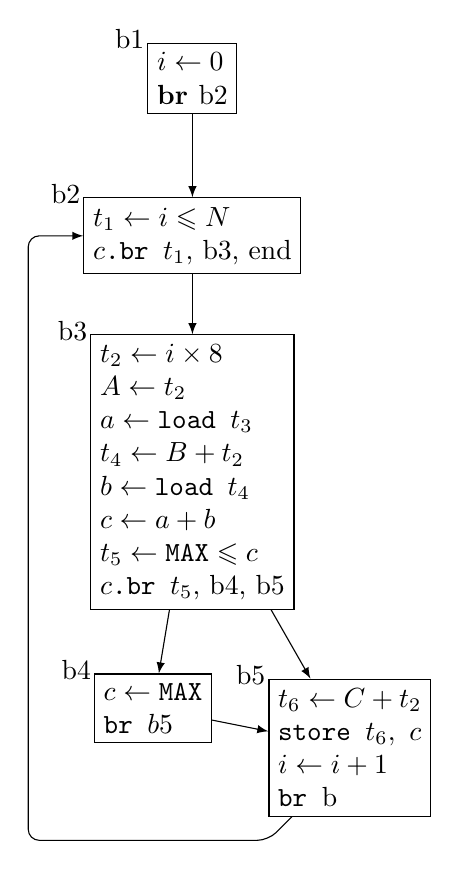
\begin{tikzpicture}[
  %, node distance = 5mm
%  start chain = going below,
  , box/.style = {draw
    %,rounded corners
    %, blur shadow
    , fill=white
    %, on chain
    , align=left
}]

  \node[box] at (0, 3) (b1) {
      $\assn{i}{0}$\\
      \textbf{br }b2
  };
  \node[box] at (0, 1) (b2) {
      $\assn{t_1}{i\leqslant N}$\\
      \cbr $t_1$, b3, end
  };
  \node[box] at (0, -2) (b3) {
    $\assn{t_2}{i\times 8}$\\
                $\assn{A}{t_2}$\\
                $\assn{a}{\load t_3}$\\
                $\assn{t_4}{B + t_2}$\\
                $\assn{b}{\load t_4}$\\
                $\assn{c}{a+b}$\\
                $\assn{t_5}{\texttt{MAX}\leqslant c}$\\
                \cbr $t_5$, b4, b5
  };
  \node[box] at (-0.5, -5) (b4) {
    $\assn{c}{\texttt{MAX}}$\\
    \br$b5$
  };
  \node[box] at (2, -5.5) (b5) {
    $\assn{t_6}{C+t_2}$\\
    \store$t_6,\ c$\\
    $\assn{i}{i+1}$\\
    \br b
  };
    \lab{1}     \lab{2} \lab{3} \lab{4}  \lab{5}
% \mynode{4}{$\assn{c}{\texttt{MAX}}$\\\br$b5$}
%    {at (3,-20)}
% \mynode{5}{$a<N$\\
%            \store$t_6, c$\\
%        	$\assn{i}{i+1}$\\
%            \br b2}
%        {at (0,-10)}

 \begin{scope}[rounded corners,-latex]
  \path %(b3.-40) edge[bend right=50] (b4.40)
    (b1) edge (b2) ;
  \path (b2) edge (b3);
  \path (b3) edge (b4);
  \path (b3) edge (b5);
  \path (b4) edge (b5);
  %\path (b5) edge (b6);
  \draw (b5.230) -- ++(-.3,-0.3) -| ([xshift=-7mm]b2.west) --
 (b2);
 \end{scope}
\end{tikzpicture}
\end{document}